\documentclass[a4paper, 12pt]{article}
\usepackage[top=2cm, bottom=2cm, left=2.5cm, right=2.5cm]{geometry}
\usepackage[utf8]{inputenc}
\usepackage[brazilian]{babel}
\usepackage{indentfirst}
\usepackage{graphicx}
\usepackage{wrapfig}
\usepackage{xcolor}
\usepackage[pdftex]{hyperref}
\graphicspath{ {imagens/} }

\begin{document}
%
\begin{titlepage} %iniciando a "capa"
	\begin{center} %centralizar o texto abaixo
		{\large Unicamp}\\[0.2cm] %0,2cm é a distância entre o texto dessa linha e o texto da próxima
		{\large Mecânica dos Fluidos}\\[0.2cm] % o comando \\ "manda" o texto ir para próxima linha
		{\large Mazza}\\[3.2cm]
		{\bf \huge Mecânica dos Fluidos}\\[0.2cm] 
		{\bf \large I}\\[4.9cm]
		% o comando \bf deixa o texto entre chaves em negrito. O comando \huge deixa o texto enorme
	\end{center} %término do comando centralizar
	{\large Erik Yuji Goto}\\[10cm] % o comando \large deixa o texto grande
	\begin{center}
		{\large Campinas}\\[0.2cm]
		{\large 2021}
	\end{center}
\end{titlepage} %término da "capa"


\tableofcontents
\newpage

\section{Conceitos Fundamentais}
	\textbf{Fluido:} É uma substância que se deforma continuamento quando submetida a uma tensão de cisalhamento, não importa o quão pequena essa tensão.\\
	
	\textbf{Composição do fluido:} Inúmeras moléculas em movimento. Vamos tratar o fluido como contínuo.\\
	
	\textbf{Referencial Lagrangiano:} Acompanha elementos de massa identificáveis.\\
	
	\textbf{Referencial Euleriano:} Focaliza a atenção sobre as propriedades do escoamento num determinado ponto do espaço como função do tempo.
	
\subsection{Tensão}
	\textbf{Tensão:} Força de superfície com duas componentes:
	\begin{itemize}
		\item Normal, também chamada de pressão;
		\item Cisalhamento, única que causa deformação no fluido.
	\end{itemize}
\subsubsection{Tensão de Deformação}
	É a variação de um ponto N em relação ao tempo.
	É um fenômeno local.
	\begin{figure}[h]
		\centering
		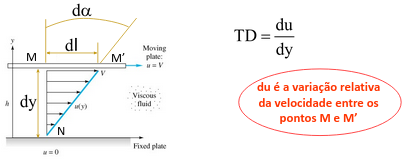
\includegraphics[width=0.7\linewidth]{imagens/tensao}
		\caption{Tensão de Deformação}
		\label{fig:tensao}
	\end{figure}
\subsubsection{Tensão x Deformação}
	Para fluidos Isaac Newton propôs:
	\begin{center}
		\Large
		$ \tau = \frac{d\mu}{dy} $
	\end{center}
	$\mu[\frac{N.s}{m^2}]$ viscosidade dinâmica\\
	
	\textbf{Fluido Newtoniano:} A viscosidade só poderá ser alterada com a temperatura;
	A relação $\tau = \frac{\mu du}{dy}$ é um modelo.
	
	\textbf{Cisalhamento Simples:} É quando a deformação é constante:
	\begin{center}
		\Large
		$
		\frac{du}{dy} = cte \rightarrow u = a.y+b
		$
	\end{center}

	\textbf{Condição de não deslizamento:} O fluido não desliza na interface com uma fronteira sólida, mas fica derido a ela.\\
	
	\textbf{Tensão Superficial:} É a força por unidade de comprimento devido à atração molecular ao longo de qualquer linha de interface.
	
\newpage
\section{Estática dos Fluidos}
	Trata do estado de forças no fluido na ausência de movimento relativo entre suas partículas.
	Implica na existência de somente tensões normais.
\subsection{Lei de Stervin}
	"A diferença de pressão entre dois pontos de massa de um líquido em equilíbrio é igual à diferença de nível entre os pontos, multiplicada pelo peso específico do líquido". Temos isso para \textbf{um mesmo fluido e mesma altura}.\\
	
	\textbf{Peso devido a coluna de água:}
	\begin{center}
		\Large
		$
		(P_{B} - P_{A}) = \varphi .g.h
		$
	\end{center}
\subsection{Referencial não Inercial}
	\begin{figure}[h]
		\centering
		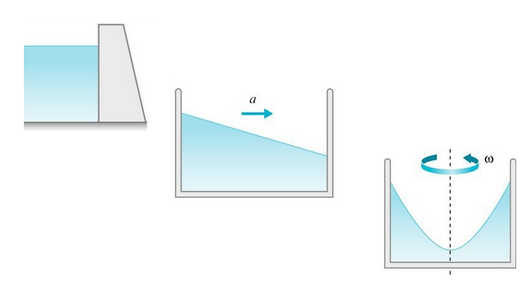
\includegraphics[width=0.7\linewidth]{imagens/aa}
		\caption[]{Aplicações}
		\label{fig:aa}
	\end{figure}
	
	\begin{center}
		\Large
		$
		- \bigtriangledown P = \rho.(\vec{g} - \vec{a}_{rel})
		$
	\end{center}
	\begin{figure}[h]
		\centering
		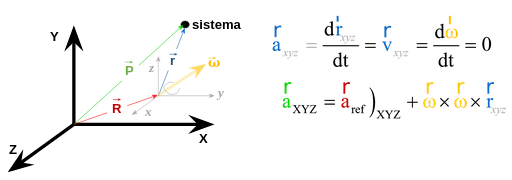
\includegraphics[width=0.7\linewidth]{imagens/aa1}
		\caption{Aceleração Relativa}
		\label{fig:aa1}
	\end{figure}
	Podemos calcular a angulação:
	\begin{center}
		\Large
		$
		\frac{dz}{dx} = - \frac{a_x}{g + a_z} = - tg \theta
		$
	\end{center}
\subsubsection{Superfícies em Rotação}
	\begin{center}
		\Large
		$
		\bigtriangledown P = - \rho g_k + \rho \omega ^2 r_r
		$
	\end{center}	
	Inclinação de superfícies em rotação:
	\begin{center}
		\Large
		$
		\alpha = arctan(\frac{\omega ^2 r}{g})
		$
	\end{center}
	\begin{figure}[h]
		\centering
		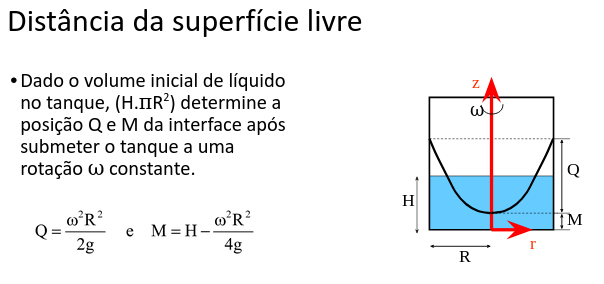
\includegraphics[width=0.8\linewidth]{imagens/aa2}
		\caption{Distância da Superfície Livre}
		\label{fig:aa2}
	\end{figure}
	

\newpage
\section{Teorema de Transporte de Reynolds}
\subsection{Conservação de Massa}
	\begin{center}
		\Large
		$
		0 = \frac{\delta}{\delta t} \int_{VC}\varphi dV + \int_{SC} \varphi \vec{V} \vec{n} dA 
		$
	\end{center}
	O termo $\vec{V}.\vec{n}$
	\begin{figure}[h]
		\centering
		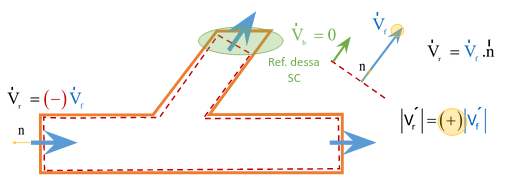
\includegraphics[width=0.7\linewidth]{imagens/rey}
		\caption{Conservação Massa}
		\label{fig:rey}
	\end{figure}
	
\subsection{Conservação de Quantidade de Movimento - Referencial Inercial}
	\begin{center}
		\Large
		$
		\frac{\delta}{\delta t}\int_{vc} \vec{V}.\varphi dV + \int_{sc}\vec{V}. \varphi. \vec{V_{r}}.\vec{n}dA = \int_{vc} \varphi.\vec{g}dV + \int_{sc}(-\vec{n}.P)dA+\int_{sc}\vec{n}.\tau dA + \vec{F_{mec}}
		$
	\end{center}
\begin{figure}[h]
	\centering
	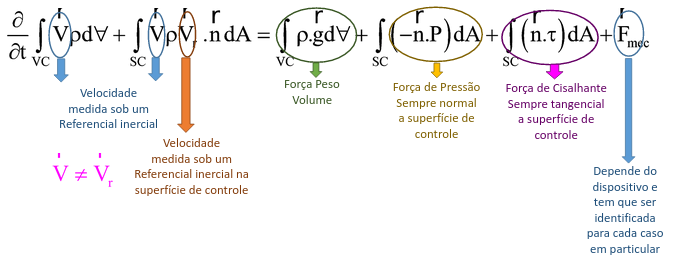
\includegraphics[width=0.5\linewidth]{imagens/eq}
	\caption{Quantidade de Movimento}
	\label{fig:eq}
\end{figure}
	Por ser uma equação vetorial ela pode ser decomposta nas três direções (\textit{x, y, z})

\subsection{Conservação de Quantidade de Movimento - Referencial Não Inercial}
	\begin{center}
		\Large
		$
		\frac{\delta}{\delta t}\int_{vc}\textcolor{blue}{\vec{v_{xyz}}}.\varphi dV + \int_{vc}\textcolor{blue}{\vec{v_{xyz}}}\varphi.\vec{V_{r}} .\vec{n}dA = \sum F_{ext} - \int_{vc} \textcolor{red}{\vec{a_{ref}}} .\varphi dV   
		$
	\end{center}
	$\textcolor{blue}{\vec{v_{xyz}}}$ é medido a partir do referencial não inercial.
\subsection{Conservação do Momento da Quantidade de Movimento}
	\begin{center}
		\Large
		$
		\int_{sc}(\vec{r_{xyz}}\times \vec{v_{xyz}})\varphi .\vec{V_{r}}.\vec{n} dA = \dot{T}_{eixo} - \int_{sc} \varphi .(\vec{r_{xyz}}\times \vec{a_{rel}})dV
		$\\
		Aceleração relativa:\\
		$
		\vec{a_{rel}} = \frac{d \vec{\omega}}{dt} \times \vec{r}_{xyz} + \vec{\omega} \times (\vec{\omega} \times \vec{r_{xyz}}) + 2\vec{\omega} \times \vec{V_{xyz}}
		$\\
		Potência\\
		$
		\dot{W}_{eixo} = T_{eixo}. \omega
		$
		
	\end{center}
\textbf{Obs:} Como o torque \textbf{T} sempre está na direção $\hat{z}$, os produtos vetoriais devem ser na mesma direção, caso contrário podemos descartá-los.

\subsection{Conservação de Energia}
	\begin{center}
		\Large
		$
		\dot{Q_{vc}} - \dot{W_{vc}} = \frac{\delta}{\delta t} \int_{vc} \varphi (u + \frac{V_I^2}{2} + g.z)dV+ \int_{sc}(\textcolor{red}{u + P.v} + \frac{V_I^2}{2}+g.z)\varphi \vec{V_r}.\vec{n}dA
		$
	\end{center}
	\textcolor{red}{*} Entalpia - h\\
	\textcolor{red}{*} As diferenças de energia cinética devem ser medidas a partir de um referencial inercial.
	
\subsection{Trabalho da Bomba}
	O papel da bomba é transferir energia para os termos mecânicos e também para as irreversibilidades.
	\begin{center}
		\Large
		$
		w_{shaft} = (\frac{V_I^2}{2} + g.z + \frac{P}{\varphi})_{in} - [(\frac{V_I^2}{2} + g.z + \frac{P}{\varphi} )_{out} + w_{irr}]
		$ ou\\
		$
		\frac{w_{shaft}}{g} = (\frac{V_I^2}{2g} + z + \frac{P}{\varphi .g})_{in} - (\frac{V_I^2}{2g} + z + \frac{P}{\varphi .g} )_{out} - h_{irr}
		$
	\end{center}

\subsection{Eq. de Bernoulli}
	Considerando um processo:
	\begin{itemize}
		\item Reversível $\longrightarrow s_{ger} = 0$;
		\item Sem transferência de Calor $\longrightarrow s_{in} = s_{out}$;
		\item Sem realização de trabalho $\longrightarrow W_{shaft} = 0$.
	\end{itemize}

	\begin{center}
		\Large
		$
		0 = (\frac{V_I^2}{2} + g.z + u + \frac{P}{\varphi})_{in} - (\frac{V_I^2}{2} + g.z + u + \frac{P}{\varphi} )_{out}
		$
	\end{center}

\section{Análise Dimensional}
\subsection{Protótipo x Modelo}
	\textbf{Protótipo:}
	Tamanho real, custo elevado e nem sempre é possível de ser realizado;\\
	
	\textbf{Modelo:}
	Tamanho escalado, custo reduzido, mas necessita de formas de inferir os resultados ao tamanho real;

\subsection{Dimensões de Algumas Grandezas Físicas}
\begin{figure}[h]
	\centering
	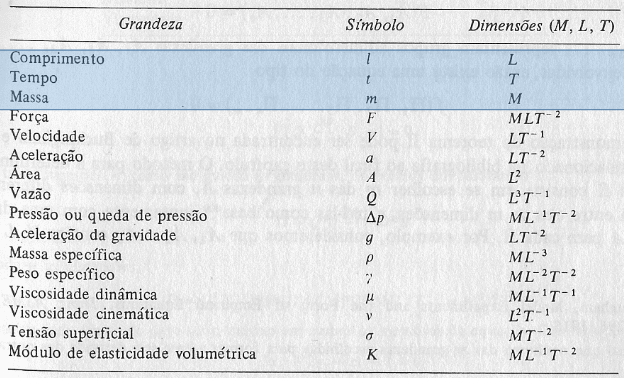
\includegraphics[width=0.9\linewidth]{imagens/dim}
	\caption{Dimensões}
	\label{fig:dim}
\end{figure}

\subsection{Teorema dos $\pi$ de Buckingham}
	O Teorema dos $\pi$ diz quantas variáveis adimensionais são requeridas para um dado conjunto de variáveis dimensionais de um dado problema.
\subsubsection{Matriz Dimensional}
	É formada listando os expoentes (a, b, c, d, etc) das dimensões primárias (M, L e T) de cada variável.
	\begin{figure}[h]
		\centering
		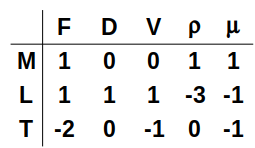
\includegraphics[width=0.5\linewidth]{imagens/mat}
		\caption{Matriz Dimensional}
		\label{fig:mat}
	\end{figure}
	O propósito da matriz dimensional é checar a independência linear das variáveis dimensionais em termos das dimensões primárias escolhidas (M, L, T).
	
	
	Isto é feito determinando-se o ‘\textbf{rank}’ da matriz.
	
	O rank é o \textbf{determinante} de todas possíveis submatrizes quadradas começando-se pela maior até encontrar uma cujo determinante é não nulo.\\

	A quantidade de parâmetros adimensionais necessário para expressar a dependência funcional será de n – r variáveis (r é o rank):
	\begin{center}
		\Large
		$
		\pi_{1} = f(\pi_{2},\pi_{3},\pi_{4}...\pi_{n-r})
		$
	\end{center}
\subsubsection{Formando os $\pi$'s}
	Os $\pi$’s são formados escolhendo-se uma base de repetição
	A base contém ‘r’ variáveis dimensionais do total de ‘n’ que contenha entre elas as ‘r’ dimensões.\\
	
	As ‘r’ variáveis da base não podem ser linearmente dependentes uma das outras. A sub-matriz dos seus expoentes dimensionais tem que ser não nulo.
\subsubsection{Cuidados}
	\begin{itemize}
		\item Evitar variáveis que possam serem derivadas da outra por uma produto de potências:
			\begin{itemize}
				\item Combinação entre comprimento, L, velocidade LT-1 e aceleração LT-2 é linearmente dependente.
				Pode-se combiná-las de forma que o resultado seja adimensional!
				\item Combinação entre comprimento, L, densidade ML-3 e velocidade LT-1 é linearmente independente.
				Pode formar uma base porque qualquer que seja o produto entre elas nunca será adimensional!
			\end{itemize}
		
		\item Evitar duas propriedades físicas para compor a base.
			\begin{itemize}
				\item Ex: Viscosidade e densidade.
			\end{itemize}
	\end{itemize}

\subsubsection{Procedimento}
	\begin{enumerate}
		\item Liste todos os parâmetros envolvidos;
		\item Selecione um conjunto de dimensões fundamentais ;
		\item Liste as dimensões de todos os parâmetros em termos das dimensões primárias;
		\item Selecione da lista um número dos parâmetros que se repetem;
		\item Estabeleça equações adimensionais combinando os parâmetros;
		\item Verifique se os parâmetros são adimensionais.
	\end{enumerate}

\section{Semelhança}
	As leis de escala podem ser aplicadas desde que haja semelhança entre modelo e protótipo.\\
	
	Os testes no modelo são semelhantes ao protótipo quando:
	\begin{center}
		\Large
		$
		\pi_{2m} = \pi_{2m};\pi_{3m} = \pi_{3m};...;\pi_{km} = \pi_{km}
		$
	\end{center}
	Usando o número de Reynolds como exemplo: Precisamos garantir que o Re do modelo e do protótipo sejam iguais para assegurar a semelhança.\\
	
	Nem sempre é possível garantir a semelhança completa.
	Ao invés de se falar em semelhança ou similaridade completa, fala-se de tipos particulares de semelhança:
	\begin{itemize}
		\item Geométrica - Um modelo e um protótipo são geometricamente similares se todas as dimensões do corpo possuírem a mesma razão linear;
		\item Cinemática - A similaridade cinemática requer que as velocidades, nas três direções coordenadas, no modelo e no protótipo tenham a mesma razão linear;
		\item Dinâmica - A  similaridade dinâmica existe quando o modelo e protótipo possuem a mesma razão de comprimento, tempo e força;
		\item Térmica.
	\end{itemize}

\section{Escoamento Interno}
	\textbf{Escoamento Laminar x Turbulento}: \textit{Escoamentos laminares} são altamente ordenados, com cada partícula do fluido seguindo umas as outras de forma ordeira.
	
	\textit{Escoamentos turbulentos} são altamente desordenados, sendo difícil definir as posições das partículas instante a instante. Diz-se que o escoamento é de alguma forma caótico
	\begin{figure}[h]
		\centering
		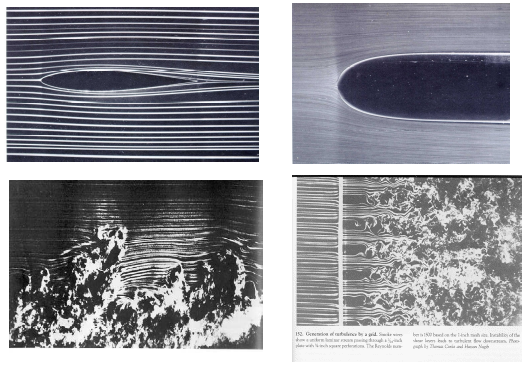
\includegraphics[width=0.7\linewidth]{imagens/escoamento}
		\caption{Escoamento Laminar e Turbulento}
		\label{fig:escoamento}
	\end{figure}
	\begin{figure}[h]
		\centering
		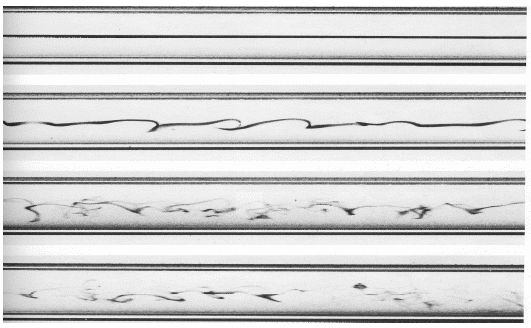
\includegraphics[width=0.7\linewidth]{imagens/escoamento1}
		\caption{Experimento de Osborne Reynolds (1841-1912)}
		\label{fig:escoamento1}
	\end{figure}

	Reynolds mostrou que para tubos as instabilidades começam quando \textbf{Re = 2.300} e que acima de \textbf{$10^4$} o escoamento é completamente turbulento.
	Entre 2.300 e $10^4$ há a \textbf{transição} do escoamento e pode haver regime laminar, turbulento ou ambas.\\
	
	Valores de Re aceitos para transição em \textbf{tubos}:
	\begin{itemize}
		\item Laminar $Re_D < 2300$
		\item Turbulento $Re_D > 4000$
		\item Transição $2300 < Re_D < 4000$
	\end{itemize}
	\begin{figure}[h]
		\centering
		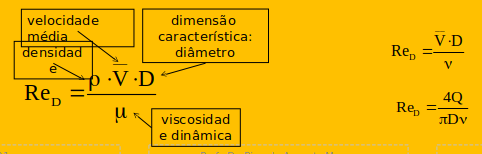
\includegraphics[width=0.7\linewidth]{imagens/re}
		\caption{Definição de Reynolds}
		\label{fig:re}
	\end{figure}

\subsection{Comprimento de Desenvolvimento}
	Enquanto que próximo  da entrada o perfil de velocidades pode ser plano, a atuação da viscosidade desacelera o fluido próximo da parede. \\
	
	Para conservar massa o núcleo deve ser acelerado!
	
	Este conjunto de fatores faz com que seja estabelecido um perfil de velocidades a jusante da entrada cujo máximo é no centro e o mínimo é na parede
	\begin{figure}[h]
		\centering
		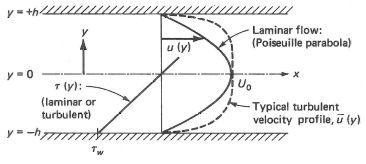
\includegraphics[width=0.7\linewidth]{imagens/des2}
		\caption{Diferença entre laminar e tubulento}
		\label{fig:des2}
	\end{figure}

	O perfil de velocidades e a pressão variam ao longo da direção axial do tubo.\\
	O comprimento da região de entrada é denominado por Le.\\
	Para distâncias superiores a Le, diz-se que o escoamento está \textbf{hidrodinamicamente desenvolvido}.
	\begin{figure}[h]
		\centering
		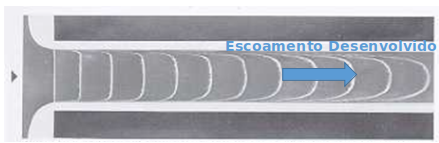
\includegraphics[width=0.7\linewidth]{imagens/des}
		\caption{Escoamento Desenvolvido}
		\label{fig:des}
	\end{figure}
	O termo ‘Desenvolvido’  significa que o perfil não mais varia ao longo da direção axial do escoamento.\\
	
	Quando o escoamento está completamente desenvolvido o vetor de velocidades é unidimensional, com apenas uma componente na direção r que depende da distância da parede.\\
	
	A pressão varia ao longo do escoamento, mas não varia transversalmente à ele, P = P(x). 
	Em qualquer seção transversal a pressão é uniforme.

\subsection{Perfil de Velocidade num Tubo}
	A velocidade não está distribuída uniformemente ao longo do tubo, mas apresenta um perfil:
	\begin{figure}[h]
		\centering
		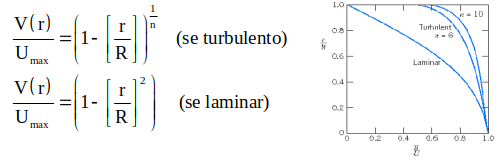
\includegraphics[width=0.7\linewidth]{imagens/vel}
		\caption{Perfil de Velocidade}
		\label{fig:vel}
	\end{figure}
	
	Num tubo a velocidade máxima, $U_{max}$, ocorre no centro (r=0). A relação entre a velocidade média e a máxima é uma função do perfil de velocidades:
	\begin{figure}[h]
		\centering
		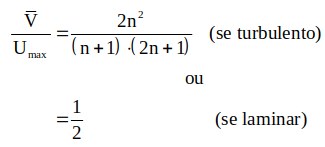
\includegraphics[width=0.6\linewidth]{imagens/vel1}
		\caption{Relação entre Velocidades}
		\label{fig:vel1}
	\end{figure}
	
\subsection{Coeficiente de Energia Cinética}
	\begin{figure}[h]
		\centering
		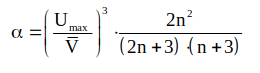
\includegraphics[width=0.4\linewidth]{imagens/coe}
		\caption{Coeficiente de Energia Cinética}
		\label{fig:coe}
	\end{figure}
	
	Para escoamentos em regime turbulento em dutos frequentemente assume-se que o coeficiente $\alpha$ é igual a 1.\\
	
	Para regime laminar entretanto é necessário o uso da correção de E.K. pois coeficiente $\alpha$ é igual a 2 
	
	\begin{itemize}
		\item Laminar: $\alpha = 2$
		\item Turbulento: $\alpha = 1$	
	\end{itemize}

	A \textbf{conservação de energia} é escrita como:
	\begin{center}
		\Large
		$
		(\alpha \frac{\bar{V}^2}{2g} + z + \frac{P}{\varphi g})_{out} - (\alpha \frac{\bar{V}^2}{2g} + z + \frac{P}{\varphi g})_{in} = -h_L - w_{eixo}
		$\\ou\\
		
		$
		w_{shaft} = (\alpha \frac{\bar{V}^2}{2} +gz + \frac{P}{\rho})_{in} - [(\alpha \frac{\bar{V}^2}{2} + gz + \frac{P}{\rho})_{out} + h_L]
		$
	\end{center}
	Obs: 
		$\dot{W}_{eixo}= \rho .Q.w_{eixo} $
	
\subsection{Introdução Perda de Carga Localizada e Distribuída}
	As perdas de carga tem origem no atrito que a parede exerce no fluido e na mudança de padrão do escoamento.\\
	 
	Desta forma, associa-se a perda de carga à uma parcela distribuída (hf) ao longo de toda tubulação e outra localizada (hm) em acessórios (curva, restrição, válvula, etc).
	\begin{center}
		\Large
		$
		h_{L} = h_{f} + \sum h_m
		$
	\end{center}



\newpage
\subsection{Perda de Carga Distribuída}
	\begin{center}
		\Large
		$
		h_{f} = f(\frac{L}{D}).(\frac{V^2}{2g}) = 8.f\frac{LQ^2}{\pi^2D^5g}[m]
		$\\$
		h_{f} = 8.f\frac{LQ^2}{\pi^2D^5}[J]
		$
	\end{center}
	\textit{f} é determinado pelo Diagrama de Moody.
\subsubsection{Rugosidade Relativa}
	\begin{figure}[h]
		\centering
		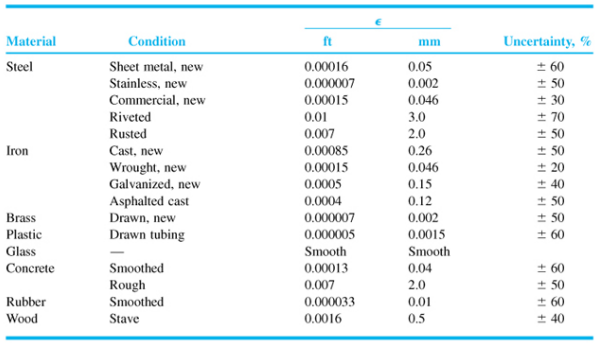
\includegraphics[width=0.7\linewidth]{imagens/rug}
		\caption{Rugosidade}
		\label{fig:rug}
	\end{figure}
	\begin{center}
		\Large
		$
		[rugosidade\cdot relativa] = \frac{\varepsilon}{d} = \frac{[rugosidade-mm]}{[diametro-tubo-mm]}
		$
	\end{center}
\subsubsection{Diagrama de Moody}
	\begin{figure}[h]
		\centering
		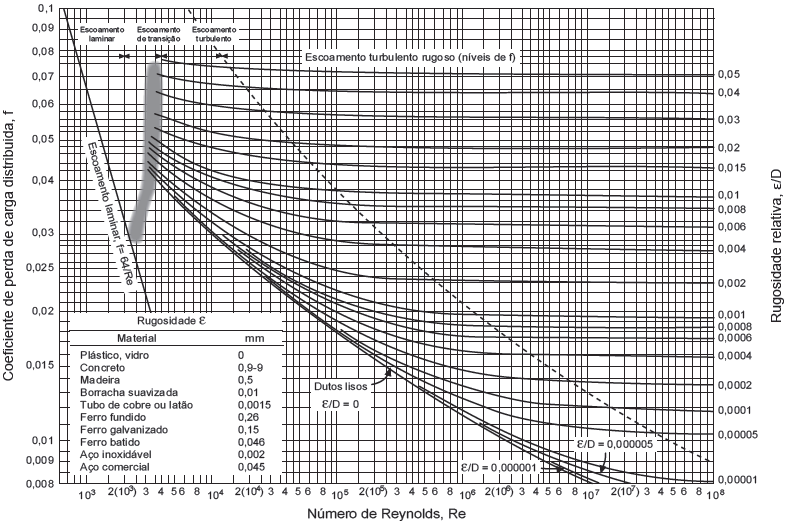
\includegraphics[width=0.9\linewidth]{imagens/moody}
		\caption{Diagrama de Moody}
		\label{fig:moody}
	\end{figure}
\subsubsection{Equação de Colebrook-White}
	O diagrama de Moody é uma representação gráfica da equação de Colebrook-White;
	\begin{center}
		$
		\frac{1}{\sqrt{f}} = -2 log[\frac{\varepsilon}{3,7D}+\frac{2,51}{Re\sqrt{f}}]
		$
	\end{center}

\newpage
\subsection{Perda de Carga Localizada}
	Toda a perda de carga localizada é modelada como sendo uma parcela da energia cinética, sendo determinada como:
	\begin{center}
		\Large
		$
		h_{m} = K.\frac{\bar{V}^2}{2}
		$ ou\\
		$
		h_{m} = f.(\frac{L_{e}}{D}).\frac{\bar{V}^2}{2}
		$
	\end{center}
	\textit{$\frac{L_{e}}{D}$}, \textit{f} e \textit{K} são encontrados em tabelas
	
\subsubsection{Contrações e Expansões}
	\begin{figure}[h]
		\centering
		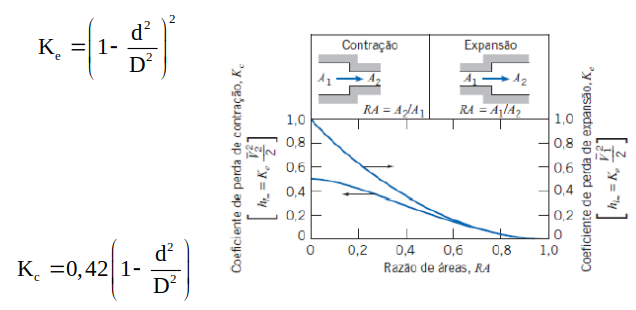
\includegraphics[width=0.7\linewidth]{imagens/cargaloc}
		\caption{Contrações e Expansões}
		\label{fig:cargaloc}
	\end{figure}

\subsubsection{Curvas, Válvulas, etc}
	\begin{figure}[h]
		\centering
		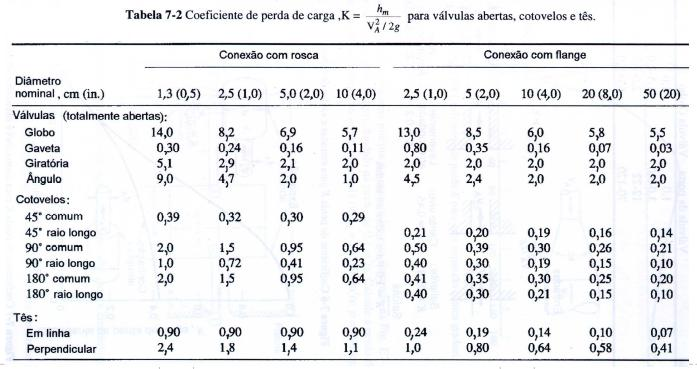
\includegraphics[width=0.9\linewidth]{imagens/valv}
		\caption{Coeficiente K}
		\label{fig:valv}
	\end{figure}

	\newpage
	\begin{figure}[h]
		\centering
		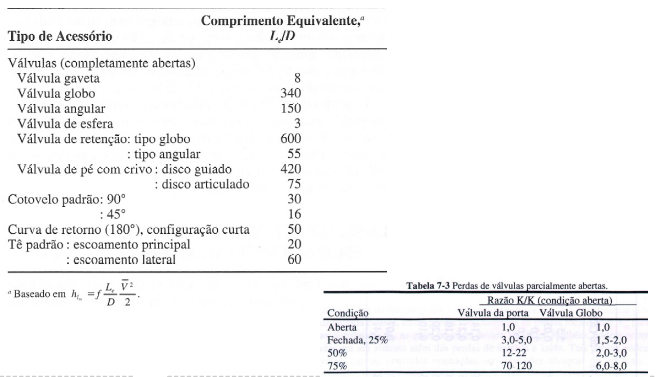
\includegraphics[width=0.9\linewidth]{imagens/valv2}
		\caption{Coeficiente $\frac{L_{e}}{D}$}
		\label{fig:valv2}
	\end{figure}
	
	\newpage
\subsubsection{Entradas e Saídas}
	\begin{figure}[h]
		\centering
		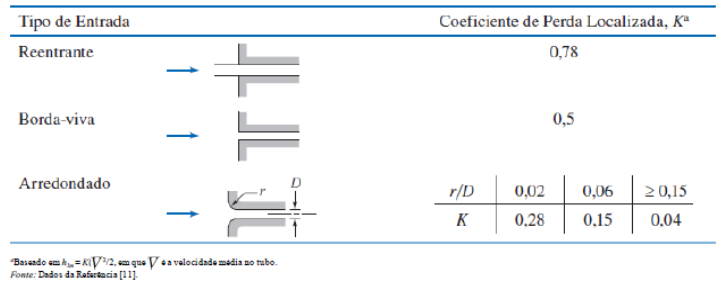
\includegraphics[width=0.9\linewidth]{imagens/valv3}
		\caption{Entradas e Saídas}
		\label{fig:valv3}
	\end{figure}
	
\subsection{Rede de Tubulações}
	De forma similar à circuitos elétricos, utilizando a leis de Kirchhoff (malha e nós), com a seguinte associação:
		\begin{itemize}
			\item Correte elétrica é similar a vazão;
			\item Diferença de potencial é similar a diferença de pressão;
			\item Resistência elétrica é similar a perda de carga:
				\begin{itemize}
					\item Resistencia elétrica é linear:
					Depende da primeira potência da corrente e é constante;
					\item Perda de carga:
					Depende do quadrado da vazão/velocidade é não é constante.
				\end{itemize}
		\end{itemize}
	
	\begin{figure}[h]
		\centering
		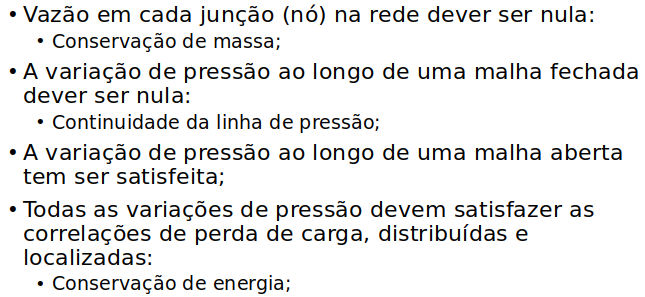
\includegraphics[width=0.8\linewidth]{imagens/regras}
		\caption{Regras}
		\label{fig:regras}
	\end{figure}
	
\newpage
\subsubsection{Exemplo}
	\begin{figure}[h]
		\centering
		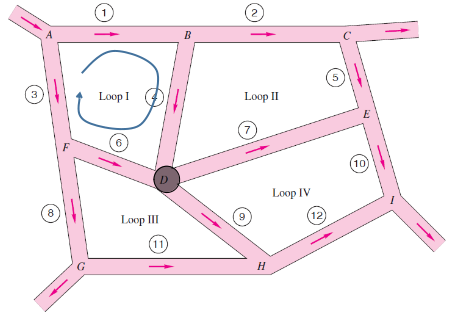
\includegraphics[width=0.8\linewidth]{imagens/rt}
		\caption{Exemplo}
		\label{fig:rt}
	\end{figure}
	\textbf{Vazão no nó D}:\\
	\begin{center}
		\Large
		$
		Q_4 + Q_6 = Q_7 + Q_9
		$
	\end{center}
	\textbf{Pressão na malha I}:\\
		\begin{center}
			\Large
			$
			P_A - P_B + P_B - P_D - (P_D - P_F) - (P_F - P_A) = 0
			$\\
			$
			P_A - P_B = f \frac{L}{D}. \frac{V^2}{2g} + \sum K \frac{V^2}{2g} - (Z_A - Z_B)
			$
		\end{center}
	Se juntarmos $(Z_A-Z_B)$ com a diferença de pressão:
		\begin{center}
			\Large
			$
			P_A - P_B = f \frac{L}{D}. \frac{V^2}{2g} + \sum K \frac{V^2}{2g} 
			$
		\end{center}
\newpage
\section{Escoamento Externo}
\subsection{Teoria da Camada Limite}
	Fora da camada limite os efeitos viscosos são desprezíveis e pode ser tratado como sem viscosidade. Equação de Bernoulli é válida!\\
	
	$\delta$ é a espessura da camada limite.
	É definida como a distância da parede onde a velocidade é de até 99\% da corrente livre.
	\begin{figure}[h]
		\centering
		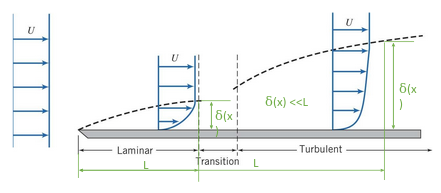
\includegraphics[width=0.7\linewidth]{imagens/ee1}
		\caption{Camada Limite}
		\label{fig:ee1}
	\end{figure}
	Na Região Interna: Efeitos viscosos e inércia são igualmente importantes. 
	Há atrito na parede e Bernoulli não pode ser usado.
	
\subsubsection{Equação Integral da Camada Limite}
	\begin{center}
		\Large
		$
		\frac{\tau_w}{\rho} = \frac{\partial}{\partial x}(U^2 \theta) + \delta^*U\frac{dU}{dx}
		$
	\end{center}
	\textbf{Espessura de Deslocamento}: Representa a espessura efetiva e está relacionada com o arrasto de pressão;\\
		\begin{center}
			$
			\delta^* = \int_{0}^{\delta}(1 - 	\frac{u}{U})dy
			$	
		\end{center}
	\begin{figure}[h]
		\centering
		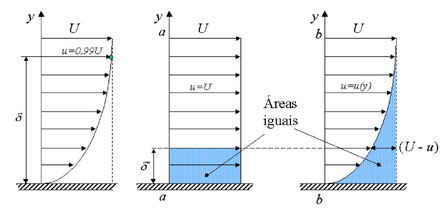
\includegraphics[width=0.7\linewidth]{imagens/a}
		\caption{Espessura de Deslocamento}
		\label{fig:a}
	\end{figure}
	\textbf{Espessura de Momento:} Pode-se dizer que a espessura de momento representa o arrasto viscoso.
		\begin{center}
			$
			\theta \approx \int_{0}^{\theta} \frac{u}{U}(1 - \frac{u}{U})dy
			$
		\end{center}
	\newpage
		\begin{figure}[h]
			\centering
			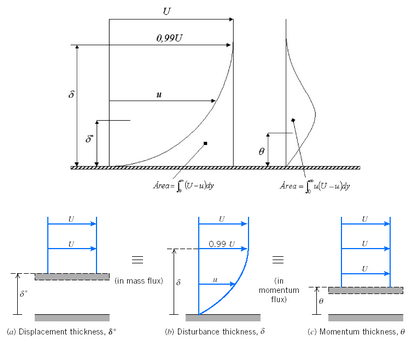
\includegraphics[width=0.7\linewidth]{imagens/a1}
			\caption{Espessura de Momento}
			\label{fig:a1}
		\end{figure}
		
\subsection{Camada Limite - Placa Plana}
	\begin{figure}[h]
		\centering
		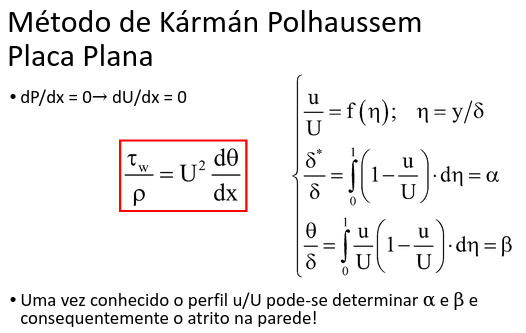
\includegraphics[width=0.6\linewidth]{imagens/a2}
		\caption{Método de Kármán Polhaussem}
		\label{fig:a2}
	\end{figure}
\newpage
\subsubsection{Placa plana: Laminar}
	\begin{figure}[h]
		\centering
		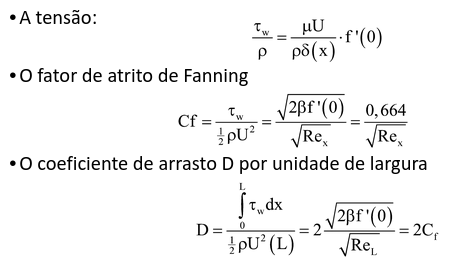
\includegraphics[width=0.7\linewidth]{imagens/pp}
		\caption{Placa Plana: Laminar}
		\label{fig:pp}
	\end{figure}

\subsubsection{Placa Plana: Turbulento}
	\begin{center}
		\Large
		$
		\frac{\delta}{x} = \frac{0,382}{Re^{1/5}_x}
		$
	\end{center}
	\textbf{Coeficiente de Atrito de Fanning}
	\begin{center}
		\Large
		$
		C_f = \frac{0,0594}{Re^{1/5}_x}
		$
	\end{center}

\section{Corpo Rombudo}
	A TCL não é válida para escoamentos com separação.
	Na separação $\delta$ cresce e $\delta$/L não é pequeno!
	Entretanto, a TCL pode prever aproximadamente o ponto de separação.
	\begin{figure}[h]
		\centering
		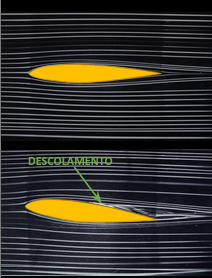
\includegraphics[width=0.5\linewidth]{imagens/sep}
		\caption{Separação do Escoamento}
		\label{fig:sep}
	\end{figure}
	O ponto de separação é definido quando  a  tensão  na  parede é nula, $\tau_w$ = 0, isto é:
		\begin{center}
			\Large
			$
			separacao \Rightarrow \frac{du}{dy} = 0
			$
		\end{center}
	\newpage
\subsection{Força Resultante no Corpo}
	\begin{figure}[h]
		\centering
		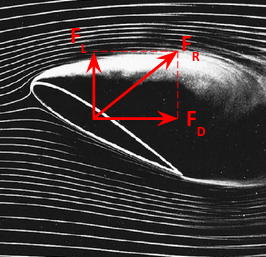
\includegraphics[width=0.7\linewidth]{imagens/sep1}
		\caption{Forças no corpo}
		\label{fig:sep1}
	\end{figure}

	A força resultante pode ser decomposta em duas componentes em relação a direção do escoamento:
	\begin{itemize}
		\item Arrasto(FD) - \textit{Paralela}
		\item Sustentação(FL) - \textit{Normal}
	\end{itemize}

\subsection{Arrasto de Forma(Presão)}
	Causa uma força resultante na direção posta ao escoamento. Ela é expressa na forma de um coeficiente:
		\begin{center}
			\Large
			$
			C_D = \frac{\bar{D}_p}{(1/2) \rho U^2_{ext} A} \longrightarrow \bar{D}_p = C_D.(\frac{1}{2}) \rho U^2_{ext}A
			$
		\end{center}
	U é a velocidade relativa, $(U_{corpo}-U_{fluido})$\\
\textbf{Arrasto total}:
	\begin{center}
		\Large
		$
		\bar{D}_T = \bar{D}_p + \bar{D}_f
		$
	\end{center}
	Para Re $\gg$ 1, o arrasto de forma $\bar{D}_p$ corresponde a maior fração do arrasto total, e o arrasto viscoso $\bar{D}_f$ pode ser desprezado.

\newpage
\subsection{Coeficiente de Sustentação}
	\begin{figure}[h]
		\centering
		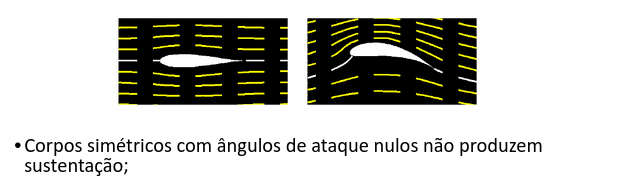
\includegraphics[width=0.8\linewidth]{imagens/sep2}
		\caption{A diferença de pressão causa a força de sustentação}
		\label{fig:sep2}
	\end{figure}
	\newpage
	\begin{figure}[h]
		\centering
		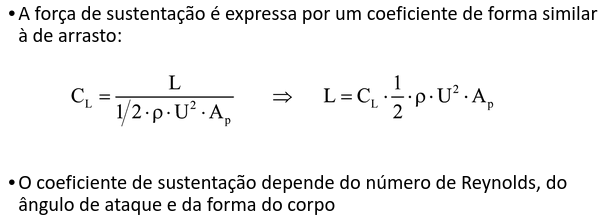
\includegraphics[width=0.7\linewidth]{imagens/sep3}
		\caption{}
		\label{fig:sep3}
	\end{figure}
	





\end{document}
	